% =====================================================================
%  Rapport - Projet BI (OLAP)
%  Compilation : pdflatex rapport.tex  (2 fois, pour la table des matières)
%  Captures : déposer les PNG dans captures/ avec les noms indiqués dans les
%  cadres "Capture à insérer", puis recompiler. Elles apparaissent toutes seules.
% =====================================================================
\documentclass[11pt,a4paper]{article}

\usepackage[utf8]{inputenc}
\usepackage[T1]{fontenc}
\usepackage{lmodern}
\usepackage[french]{babel}
\usepackage[a4paper,margin=2.2cm]{geometry}
\usepackage{graphicx}
\usepackage{float}
\usepackage{placeins}
\usepackage{booktabs}
\usepackage{tabularx}
\usepackage{array}
\usepackage{enumitem}
\usepackage{xcolor}
\usepackage{listings}
\usepackage{caption}
\usepackage[obeyspaces,spaces]{url}   % garde les espaces dans \code{...} (CRON, SQL)
\usepackage[hidelinks]{hyperref}

% Les deux-points et points-virgules "actifs" de babel-french gênent les URL JDBC
\AtBeginDocument{\shorthandoff{;:!?}}

% \code{...} : identifiants, URL, chemins (police machine, coupure de ligne autorisée)
\DeclareUrlCommand\code{\urlstyle{tt}}
\def\UrlBreaks{\do\/\do\;\do\=\do\:\do\.\do\_\do\,\do\-}

\definecolor{codebg}{gray}{0.96}
\lstset{
  basicstyle=\ttfamily\footnotesize,
  backgroundcolor=\color{codebg},
  frame=single, rulecolor=\color{gray!40},
  breaklines=true, columns=fullflexible, keepspaces=true,
  xleftmargin=4pt, xrightmargin=4pt, aboveskip=8pt, belowskip=8pt
}

\setlist{itemsep=2pt, topsep=4pt}
\renewcommand{\arraystretch}{1.25}
\newcolumntype{L}[1]{>{\raggedright\arraybackslash}p{#1}}
\newcolumntype{Y}{>{\raggedright\arraybackslash}X}

% Capture d'écran : affichée si le fichier existe dans captures/, sinon un cadre à remplir
% Pages composées uniquement de figures : figures alignées en haut (pas centrées)
\makeatletter
\setlength{\@fptop}{0pt}
\setlength{\@fpsep}{14pt}
\makeatother

% \capture[largeur]{fichier}{légende}   (largeur en fraction de \linewidth, 1 par défaut)
\newcommand{\capture}[3][1]{%
  \begin{figure}[!htbp]\centering
  \IfFileExists{captures/#2}%
    {\fbox{\includegraphics[width=#1\linewidth]{captures/#2}}}%
    {\fbox{\parbox{0.92\linewidth}{\centering\vspace{1.4em}%
      \textit{Capture à insérer : #3}\\[0.4em]%
      {\footnotesize fichier attendu : \texttt{captures/\detokenize{#2}}}\vspace{1.4em}}}}%
  \caption{#3}
  \end{figure}}

\title{\textbf{Projet BI -- Rapport}\\[0.4em]
  \large Data warehouse des ventes classicmodels et dellstore}
\author{Groupe 5\\[0.2em] Prénom NOM, Prénom NOM, Prénom NOM\\[0.3em]
  \small Business Intelligence -- Dr S.~Cremer}
\date{\today}

\begin{document}
\maketitle
\tableofcontents
\newpage

% ---------------------------------------------------------------------
\section{Contexte et architecture}

Les ventes de deux bases OLTP (classicmodels et dellstore) sont réunies chaque nuit
dans une BD OLAP en étoile, analysée dans Power BI Desktop.

\begin{figure}[H]
  \centering
  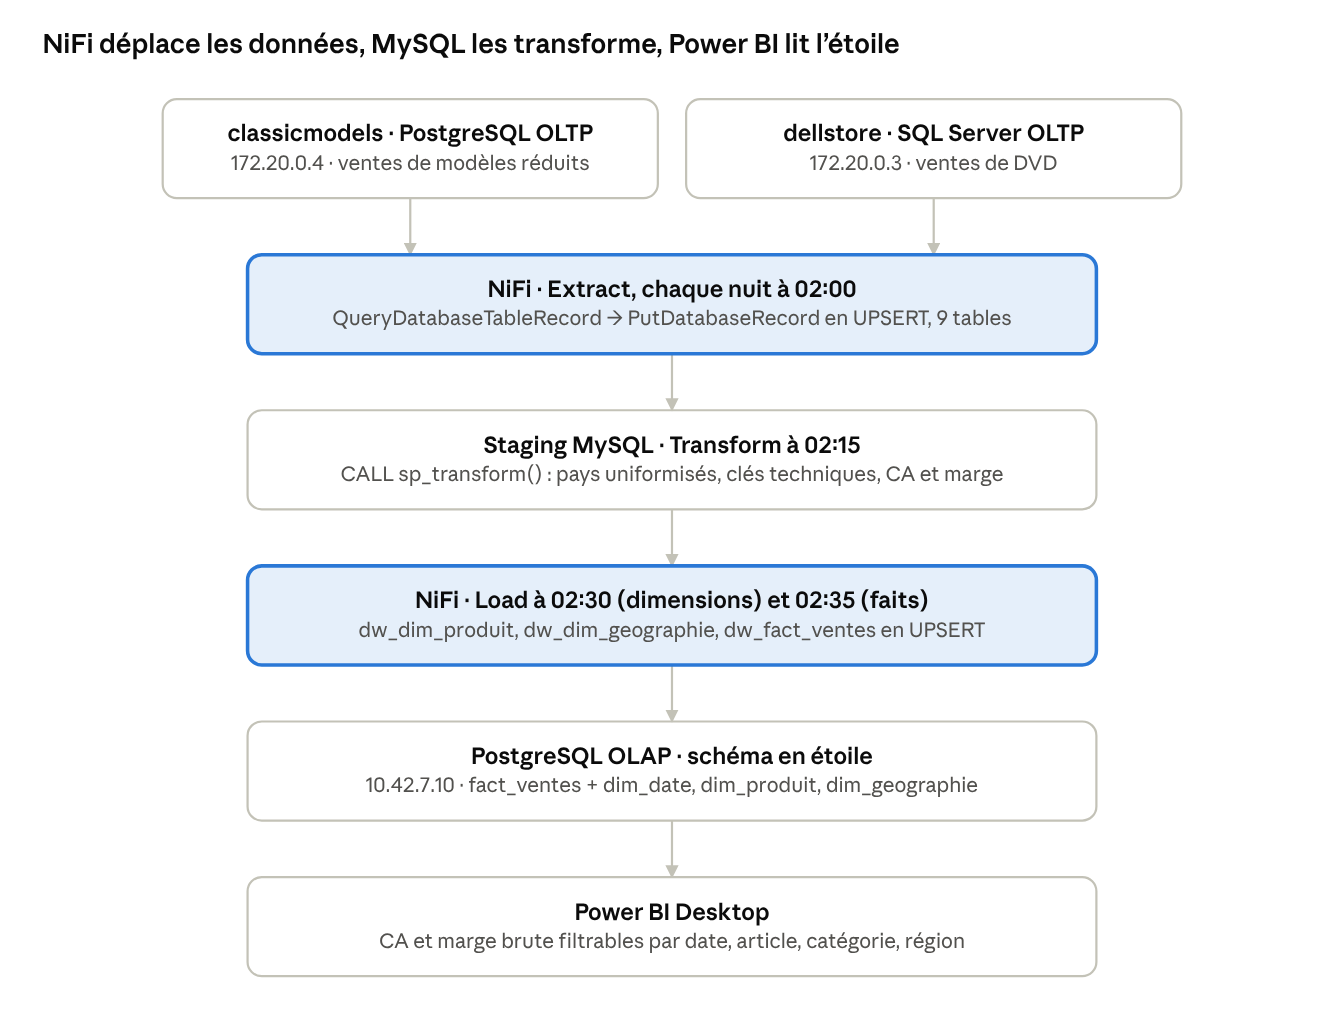
\includegraphics[width=0.82\linewidth]{figures/architecture.png}
  \caption{Architecture du projet : 2 sources, 1 ETL (NiFi), 1 staging (MySQL), 1 OLAP (PostgreSQL)}
\end{figure}

Les bases OLTP ne sont jamais modifiées : NiFi les lit, et toute la transformation se fait
dans le staging MySQL (slide 43), avant le chargement de l'OLAP.

% ---------------------------------------------------------------------
\section{Les 5 étapes d'analyse}

Le modèle retenu est une étoile au grain de la ligne de commande, avec trois dimensions :
date, produit, géographie (démarche de la slide 70).

\begin{enumerate}
  \item \textbf{Identifier le business process} : les ventes des deux sociétés (modèles réduits
  pour classicmodels, DVD pour dellstore). But : suivre le chiffre d'affaires (CA) et la marge
  brute, filtrables par date, article, catégorie d'article et région géographique.
  \item \textbf{Définir le grain} : une ligne de commande (un article dans une commande), au jour
  près. C'est le niveau le plus fin des deux sources ; tout le reste s'obtient par agrégation
  (roll-up), jamais l'inverse.
  \item \textbf{Identifier les dimensions} : Date (quand), Produit (quoi : article et catégorie),
  Géographie (où : zone, pays, état, ville du client). Date est une dimension statique générée en
  SQL ; Produit et Géographie sont des SCD type 1. Source, numéro de commande, numéro de ligne et
  statut restent dans la table de faits comme dimensions dégénérées (slide 80).
  \item \textbf{Définir les faits} : quantité, CA (quantité $\times$ prix unitaire), coût d'achat
  (quantité $\times$ coût unitaire), marge brute (CA $-$ coût d'achat). Les quatre mesures sont
  additives ; le taux de marge, non additif, est calculé dans Power BI.
  \item \textbf{Créer le schéma} : étoile, avec une table de faits et trois dimensions
  dénormalisées (la catégorie est dans \code{dim_produit}, la zone et le pays dans
  \code{dim_geographie}). Les requêtes restent simples, avec une seule jointure par dimension
  (slide 74).
\end{enumerate}

% ---------------------------------------------------------------------
\section{Schéma de la BD OLAP (étoile)}

La BD OLAP PostgreSQL contient quatre tables : \code{fact_ventes} au centre, reliée par clé
étrangère à \code{dim_date}, \code{dim_produit} et \code{dim_geographie}.

\begin{figure}[H]
  \centering
  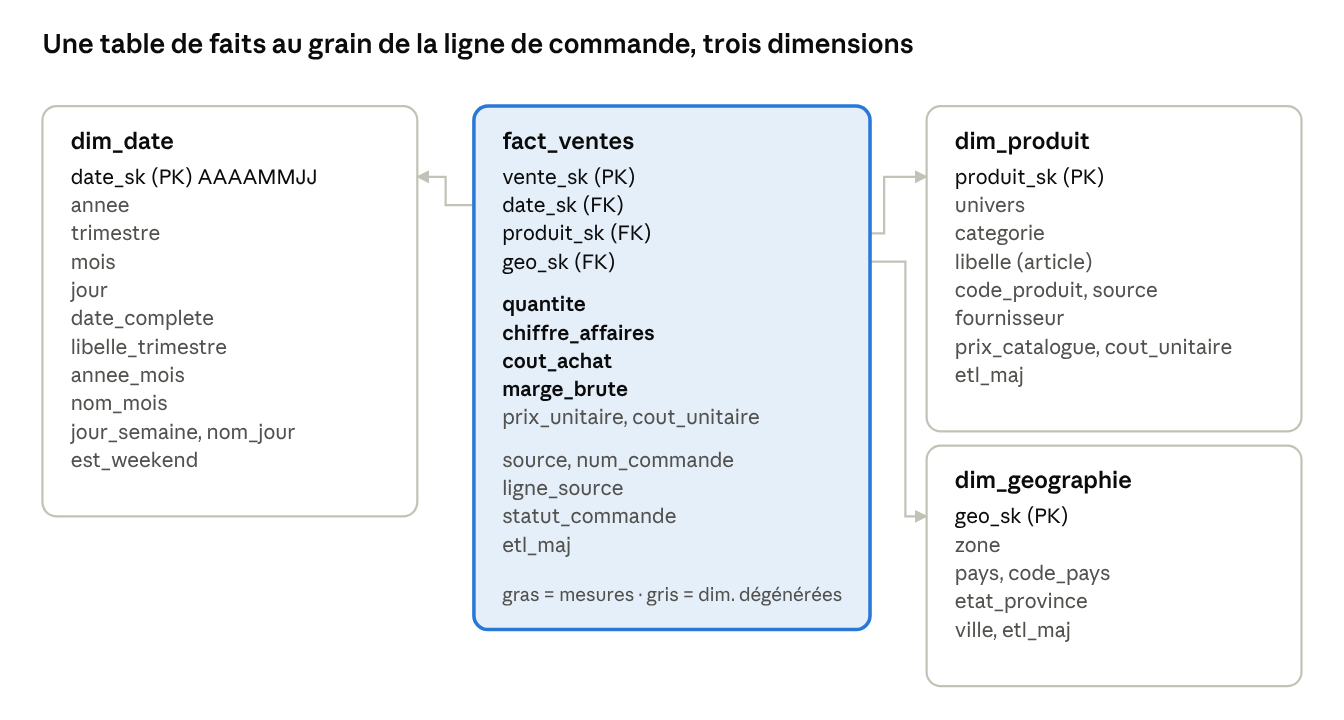
\includegraphics[width=\linewidth]{figures/schema_etoile.png}
  \caption{Schéma en étoile de la BD OLAP : 1 table de faits, 3 dimensions}
\end{figure}

Les colonnes de chaque dimension suivent leur hiérarchie (slide 69) : année $>$ trimestre $>$
mois $>$ jour, univers $>$ catégorie $>$ article, zone $>$ pays $>$ état $>$ ville. La clé de
\code{dim_date} est au format AAAAMMJJ et la table est générée par SQL de 2000 à 2030 ; les autres
clés techniques viennent du staging. Script : \code{01_olap_postgres.sql}.

% ---------------------------------------------------------------------
\section{Schéma de la BD de staging (MySQL)}

La transformation se fait dans MySQL (zone de transit, slide 43), pas dans NiFi : NiFi ne fait
que déplacer les données, et la procédure stockée \code{sp_transform} construit les tables finales.

\begin{table}[H]
\centering\footnotesize
\begin{tabularx}{\linewidth}{L{1.6cm} Y L{2.2cm} Y}
\toprule
\textbf{Groupe} & \textbf{Tables} & \textbf{Remplies par} & \textbf{Rôle} \\
\midrule
\code{stg_cm_*} & \code{stg_cm_products}, \code{stg_cm_customers}, \code{stg_cm_orders}, \code{stg_cm_orderdetails} & NiFi (UPSERT) & Copie de classicmodels, colonnes utiles uniquement \\
\code{stg_ds_*} & \code{stg_ds_categories}, \code{stg_ds_products}, \code{stg_ds_customers}, \code{stg_ds_orders}, \code{stg_ds_orderlines} & NiFi (UPSERT) & Copie de dellstore, colonnes utiles uniquement \\
\code{ref_*} & \code{ref_pays}, \code{ref_taux_cout_ds}, \code{etl_parametre} & Script SQL 02 & Correspondance pays $\rightarrow$ nom unique + zone ; taux de coût dellstore \\
\code{v_clients} & Vue & -- & Clients des 2 sources avec une géographie uniformisée \\
\code{dw_*} & \code{dw_dim_produit}, \code{dw_dim_geographie}, \code{dw_fact_ventes} & \code{sp_transform} & Contenu final de l'OLAP, avec les clés techniques (AUTO\_INCREMENT) \\
\code{etl_*} & \code{etl_controle}, \code{etl_journal} & \code{sp_transform} & Watermark du CDC, journal de chaque exécution \\
\bottomrule
\end{tabularx}
\caption{Tables de la BD de staging}
\end{table}

Chaque table \code{stg_} et \code{dw_} porte une colonne
\code{etl_maj DATETIME(3) ... ON UPDATE CURRENT_TIMESTAMP(3)}. MySQL ne la met à jour que si une
valeur de la ligne change réellement : c'est elle qui repère les lignes modifiées (CDC).
Scripts : \code{02_staging_mysql.sql} (tables, références, vue) et \code{03_transform_mysql.sql}
(procédure).

% ---------------------------------------------------------------------
\section{Flux réalisé dans NiFi}

Le process group \og Projet BI \fg{} contient 4 sous-groupes, soit 26 processeurs, déclenchés
chaque nuit dans l'ordre Extract $\rightarrow$ Transform $\rightarrow$ Load.

\begin{figure}[H]
  \centering
  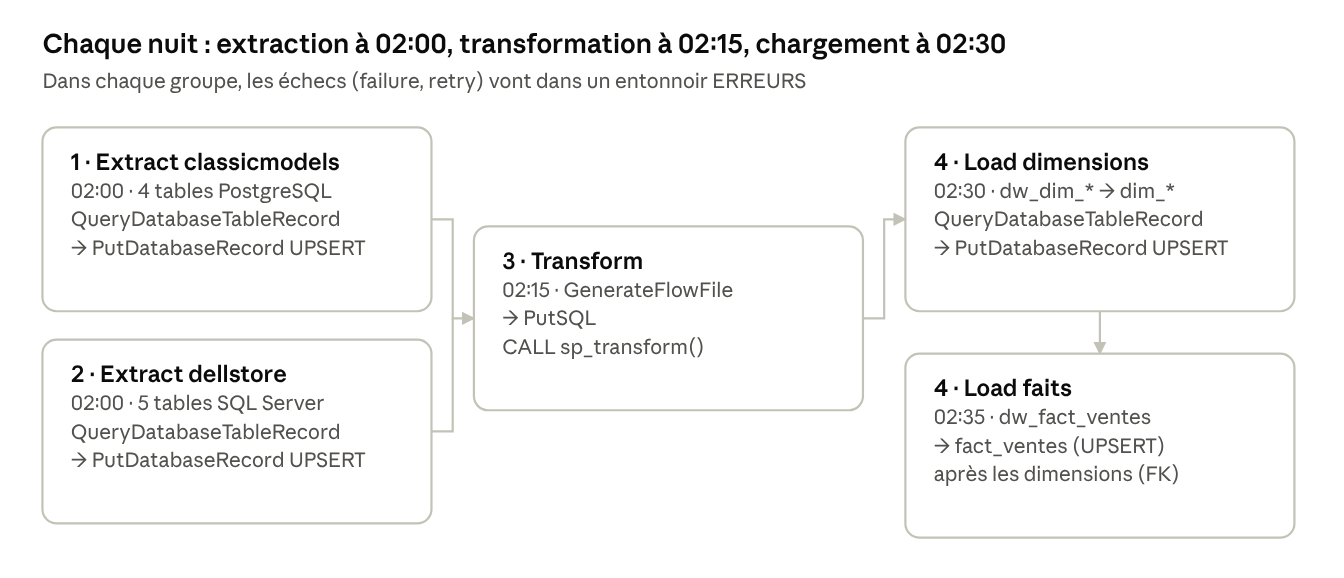
\includegraphics[width=\linewidth]{figures/flux_nifi.png}
  \caption{Flux NiFi : 4 process groups planifiés en CRON}
\end{figure}

Le décalage horaire garantit l'ordre : les dimensions arrivent dans l'OLAP avant les faits qui
les référencent. Pour une démonstration, on lance chaque groupe à la main (clic droit $>$ Run Once)
dans le même ordre. Le flux complet est fourni dans \code{flux_projet_bi.json}, à importer dans NiFi.
Les captures NiFi ci-dessous viennent du NiFi de l'école (version 1.23.1, groupe 5). Elles ont été
prises juste après une exécution complète du flux sur les vraies bases : 106\,966 lignes extraites
des deux OLTP et 64\,106 ventes chargées dans l'OLAP en 1~min~25~s, sans aucune erreur.

\capture[0.52]{nifi_global.png}{Vue d'ensemble du process group Projet BI}
\capture[0.86]{nifi_groupe1.png}{Intérieur du groupe 1 - Extract classicmodels}

% ---------------------------------------------------------------------
\section{Configuration des processeurs}

Les connexions sont des controller services du groupe \og Projet BI \fg. Leurs URL, logins et
mots de passe viennent du contexte de paramètres \og Projet BI - connexions \fg.

\begin{table}[H]
\centering\footnotesize
\begin{tabularx}{\linewidth}{L{3.1cm} Y}
\toprule
\textbf{Controller service} & \textbf{URL / classe du driver / emplacement du driver} \\
\midrule
DBCP classicmodels & \code{jdbc:postgresql://172.20.0.4:5432/classicmodels}\newline
  \code{org.postgresql.Driver}\newline \code{/opt/nifi/drivers/postgresql-42.6.0.jar} \\
DBCP dellstore & \code{jdbc:sqlserver://172.20.0.3:1433;encrypt=false;databaseName=dellstore;integratedSecurity=false;}\newline
  \code{com.microsoft.sqlserver.jdbc.SQLServerDriver}\newline \code{/opt/nifi/drivers/mssql-jdbc-12.4.0.jre8.jar} \\
DBCP staging & \code{jdbc:mysql://172.20.0.65:3306/user_ktm}\newline
  \code{com.mysql.cj.jdbc.Driver}\newline \code{/opt/nifi/drivers/mysql-connector-j-8.1.0.jar} \\
DBCP OLAP & \code{jdbc:postgresql://10.42.7.10:5432/user_ktm}\newline
  \code{org.postgresql.Driver}\newline \code{/opt/nifi/drivers/postgresql-42.6.0.jar} \\
AvroRecordSetWriter, AvroReader & Valeurs par défaut (schéma Avro embarqué) \\
\bottomrule
\end{tabularx}
\caption{Controller services}
\end{table}

\begin{table}[H]
\centering\footnotesize
\begin{tabularx}{\linewidth}{L{3.3cm} Y L{3.2cm}}
\toprule
\textbf{Processeur (nombre)} & \textbf{Propriétés modifiées} & \textbf{Planification} \\
\midrule
QueryDatabase\-TableRecord, extraction (9) & Database Type = PostgreSQL ou MS SQL 2012+ ; Table Name ;
  Columns to Return (classicmodels) ou Custom Query (dellstore) ; Maximum-value Columns = \code{last_update} ;
  Record Writer = AvroRecordSetWriter ; Use Avro Logical Types = true & CRON \code{0 0 2 * * ?} \\
PutDatabaseRecord, vers le staging (9) & Record Reader = AvroReader ; Database Type = MySQL ;
  Statement Type = UPSERT ; DBCP staging ; Table Name = \code{stg_...} ;
  Unmatched Column Behavior = Ignore Unmatched Columns & En continu ; success auto-terminé ;
  failure et retry vers l'entonnoir ERREURS \\
GenerateFlowFile (1) & Custom Text = \code{CALL sp_transform();} (simple déclencheur) & CRON \code{0 15 2 * * ?} \\
PutSQL (1) & JDBC Connection Pool = DBCP staging ; SQL Statement = \code{CALL sp_transform()} & En continu \\
QueryDatabase\-TableRecord, lecture \code{dw_} (3) & Database Type = MySQL ; Table Name = \code{dw_...} ;
  Maximum-value Columns = \code{etl_maj} & Dimensions \code{0 30 2 * * ?}, faits \code{0 35 2 * * ?} \\
PutDatabaseRecord, vers l'OLAP (3) & Database Type = PostgreSQL ; Statement Type = UPSERT ; DBCP OLAP ;
  Table Name = \code{dim_produit}, \code{dim_geographie}, \code{fact_ventes} ;
  Update Keys = \code{produit_sk}, \code{geo_sk}, \code{vente_sk} & En continu \\
\bottomrule
\end{tabularx}
\caption{Processeurs NiFi}
\end{table}

Exemple de Custom Query dellstore (la date de modification vient de la table \code{hist_}) :

\begin{lstlisting}[language=SQL]
SELECT ol.orderid, ol.orderlineid, ol.prod_id, ol.quantity, ol.orderdate,
       COALESCE(h.last_update, CAST('1900-01-01' AS DATETIME2(3))) AS last_update
FROM orderlines ol
LEFT JOIN hist_orderlines h ON h.orderid = ol.orderid AND h.orderlineid = ol.orderlineid
\end{lstlisting}

\capture[0.78]{nifi_config_qdtr.png}{Fenêtre Configure d'un QueryDatabaseTableRecord (Extract orderdetails)}
\capture[0.78]{nifi_config_pdr.png}{Fenêtre Configure d'un PutDatabaseRecord (Upsert stg\_cm\_orderdetails)}

% ---------------------------------------------------------------------
\section{Règles de transformation}

La procédure \code{sp_transform} applique les règles suivantes dans une seule transaction
(tout ou rien) :

\begin{itemize}
  \item \textbf{Uniformisation des pays} (slides 46 et 48) : la table \code{ref_pays} ramène
  \og USA \fg{} et \og US \fg{} à United States, \og UK \fg{} à United Kingdom, et \og Norway \fg{}
  suivi d'espaces à Norway. Chaque pays reçoit une zone : Europe, Amérique du Nord, Amérique latine,
  Asie-Pacifique, Afrique ou Moyen-Orient. Les clients dellstore viennent de 246 pays : \code{ref_pays}
  contient donc la liste mondiale complète (262 libellés). Un pays inconnu recevrait la zone
  \og Autre \fg{} ; après chargement, aucun client n'est dans ce cas.
  \item \textbf{Champs vides} : un état ou une ville vide devient \og N/A \fg, et un statut absent
  (dellstore) \og Non renseigné \fg.
  \item \textbf{Clés} : chaque ligne de dimension reçoit une clé technique, et la clé métier
  (source + code) est unique. Le produit 1 de dellstore ne peut donc pas être confondu avec un
  produit classicmodels. Une vente est identifiée par (source, numéro de commande, ligne).
  \item \textbf{CA et coût classicmodels} : CA = \code{quantityordered} $\times$ \code{priceeach}
  (le prix réel de la ligne), coût = \code{quantityordered} $\times$ \code{buyprice}.
  \item \textbf{CA et coût dellstore} : \code{orderlines} n'a pas de prix, donc
  CA = \code{quantity} $\times$ \code{products.price}. dellstore n'a \textbf{aucun prix d'achat} :
  le coût est estimé à 65\,\% du prix de vente. Ce taux est réglable dans \code{etl_parametre},
  ou par catégorie dans \code{ref_taux_cout_ds}.
  \item \textbf{Anonymisation} (slide 29) : aucune donnée personnelle n'est extraite (noms,
  adresses, téléphones, cartes de crédit, mots de passe). Seuls la ville, l'état et le pays du
  client sont conservés.
  \item \textbf{Commandes annulées} : elles restent dans les faits avec leur statut
  (\og Cancelled \fg) et sont exclues des mesures Power BI.
  \item \textbf{Date} : la date de commande donne \code{date_sk} au format AAAAMMJJ
  (par exemple 20040315).
\end{itemize}

% ---------------------------------------------------------------------
\section{Visualisation Power BI}

Power BI Desktop lit directement l'étoile de la BD OLAP (connecteur PostgreSQL, mode Import,
serveur \code{10.1.20.51:27171} depuis le local de cours). Le rapport est fourni sous forme de projet
Power BI (\code{powerbi/ProjetBI.pbip}) : le serveur et la base sont deux paramètres Power Query
(\code{Serveur}, \code{BaseOLAP}), modifiables sans toucher au modèle.

\paragraph{Modèle.} \code{fact_ventes} est reliée à \code{dim_date}, \code{dim_produit} et
\code{dim_geographie} par \code{date_sk}, \code{produit_sk} et \code{geo_sk} (plusieurs-à-un,
filtre à sens unique). \code{dim_date} est marquée comme table de dates sur \code{date_complete},
et \code{nom_mois} est trié par \code{mois}. Trois hiérarchies permettent le drill-down :
Année $>$ Trimestre $>$ Mois $>$ Jour, Univers $>$ Catégorie $>$ Article,
Zone $>$ Pays $>$ État $>$ Ville.

\paragraph{Mesures DAX} (les commandes annulées ne comptent pas) :

\begin{lstlisting}
CA =
CALCULATE ( SUM ( fact_ventes[chiffre_affaires] ),
            fact_ventes[statut_commande] <> "Cancelled" )

Marge brute =
CALCULATE ( SUM ( fact_ventes[marge_brute] ),
            fact_ventes[statut_commande] <> "Cancelled" )

Taux de marge = DIVIDE ( [Marge brute], [CA] )

CA N-1 = CALCULATE ( [CA], SAMEPERIODLASTYEAR ( dim_date[date_complete] ) )
\end{lstlisting}

\begin{table}[H]
\centering\footnotesize
\begin{tabularx}{\linewidth}{L{3cm} Y L{4.3cm}}
\toprule
\textbf{Visuel} & \textbf{Champs} & \textbf{Rôle} \\
\midrule
4 segments (slicers) & Période (entre deux dates), Région (Zone $>$ Pays), Catégorie et Article (listes déroulantes) & Filtres demandés : date, article, catégorie, région \\
4 cartes & CA, Marge brute, Taux de marge, Quantité vendue & Indicateurs clés \\
Courbe & Mois (\code{annee_mois}) en axe ; CA et Marge brute & Évolution dans le temps \\
Barres groupées & Catégorie ; CA et Marge brute, triées par CA & Comparaison des catégories \\
Histogramme groupé & Zone ; CA et Marge brute & Répartition par région \\
Matrice & Lignes Zone $>$ Pays, colonnes Année ; CA, Marge brute & Roll-up, drill-down et pivot (slides 57 à 61) \\
\bottomrule
\end{tabularx}
\caption{Page \og Analyse des ventes \fg}
\end{table}

Les captures ci-dessous ont été prises dans Power BI Desktop (version 2.159), connecté à la BD
OLAP de l'école. Le total de la matrice (CA 16\,006\,097, marge 6\,307\,401) correspond au contrôle
SQL de la BD OLAP, commandes annulées exclues. Filtrée sur Europe et Classic Cars, la page donne un
CA de 2\,522\,892 et une marge de 1\,018\,843, là encore identiques au SQL. Le serveur PostgreSQL
de l'école utilise un certificat auto-signé : il faut décocher \og Chiffrer les connexions \fg{}
dans les paramètres de la source de données de Power BI.

\capture[0.8]{powerbi_modele.png}{Vue Modèle : l'étoile et ses 3 relations plusieurs-à-un}
\capture{powerbi_page.png}{Page « Analyse des ventes », sans filtre}
\capture{powerbi_filtre.png}{La même page filtrée sur Europe et Classic Cars}

% ---------------------------------------------------------------------
\section{Bonus : Change Data Capture, contrôles et limites}

Le pipeline ne déplace que ce qui a changé, à chacune des trois étapes (slides 88 et 89) :

\begin{enumerate}
  \item \textbf{Extract} : QueryDatabaseTableRecord mémorise le plus grand \code{last_update} déjà
  lu. Le premier passage charge tout (initial load), les suivants uniquement les lignes plus
  récentes. classicmodels a une colonne \code{last_update} dans ses tables ; dellstore garde ses
  dates de modification dans les tables \code{hist_*}.
  \item \textbf{Transform} : \code{sp_transform} ne recalcule que les lignes dont \code{etl_maj}
  est postérieur au dernier passage (watermark dans \code{etl_controle}). Les lignes jamais
  intégrées sont aussi reprises, par sécurité. Les ventes déjà chargées ne sont jamais
  recalculées, ce qui respecte la non-volatilité (slide 23).
  \item \textbf{Load} : seules les lignes \code{dw_} dont \code{etl_maj} a changé sont envoyées
  vers l'OLAP, en UPSERT.
\end{enumerate}

\paragraph{Démonstration sur l'infrastructure de l'école.} Les deux OLTP sont partagés entre
les groupes et en lecture seule. C'est le professeur qui y ajoute des lots de modifications, le
dernier le 09/11 à 11:09 : 8 commandes et 40 lignes par source, plus quelques clients et produits
mis à jour. Ce lot a été rejoué sans toucher aux sources :
\begin{enumerate}
  \item l'entrepôt du groupe (staging et OLAP) a été remis dans son état d'avant le lot, en
  retirant ses 16 commandes et leurs 80 ventes ;
  \item le repère CDC de NiFi a été placé juste avant le lot, avec la propriété
  \code{initial.maxvalue.last_update} = \code{2026-11-09 11:00:00} ;
  \item l'ETL a ensuite été lancé normalement.
\end{enumerate}
Seul le lot a circulé. L'extraction \code{orderdetails} pèse 1,47~Ko, contre 86,79~Ko au
chargement complet. La transformation a traité exactement 40 + 40 ventes en 2,3~s. Aucune dimension
n'a été renvoyée, car les clients et produits du lot étaient déjà identiques. Les 80 ventes ont été
chargées en un seul envoi, et l'OLAP est revenu exactement aux totaux des sources. Les passages
sans changement ne recalculent rien, même après une ré-extraction complète : l'UPSERT d'une ligne
identique ne modifie pas \code{etl_maj}.

\capture[0.82]{nifi_cdc.png}{Passage incrémental dans le groupe 1 : seul le lot du 09/11 est extrait}
\capture[0.7]{cdc_ecole.png}{Rejeu du lot du 09/11 sur l'infrastructure de l'école : seul le lot circule, OLAP = sources}

Les cas que le professeur ne produit pas (quantité modifiée, commande annulée) ont été testés sur
une copie locale des deux schémas (Docker : PostgreSQL, SQL Server, MySQL et NiFi 1.28) :

\begin{table}[H]
\centering\footnotesize
\begin{tabularx}{\linewidth}{L{3cm} Y L{2.6cm} L{2.4cm}}
\toprule
\textbf{Exécution} & \textbf{Changements dans les sources} & \textbf{Ventes envoyées vers l'OLAP} & \textbf{Totaux OLAP = sources} \\
\midrule
1 (chargement initial) & -- & 701 & Oui \\
2 & Aucun & 0 & Oui \\
3 & 1 quantité modifiée, 1 commande annulée, 2 nouvelles commandes, 1 nouveau client & 7 & Oui \\
\bottomrule
\end{tabularx}
\caption{Test du CDC}
\end{table}

\paragraph{Contrôles post-chargement} (slide 49, script \code{04_controles.sql}) : CA et marge
brute recalculés dans chaque source et comparés à l'OLAP, pays non reconnus, lignes de commande
non transformées, et journal \code{etl_journal} de chaque exécution (OK ou ERREUR).

\capture[0.66]{controles.png}{Contrôles du script 04 sur les bases de l'école : totaux sources = OLAP, journal, lignes orphelines}

\FloatBarrier
\paragraph{Limites.}
\begin{itemize}
  \item La marge brute de dellstore repose sur un coût estimé (65\,\% du prix), faute de prix
  d'achat dans la source.
  \item Le prix dellstore est le prix catalogue au moment de l'intégration, car \code{orderlines}
  ne garde pas le prix payé.
  \item Une ligne supprimée physiquement dans une source n'est pas propagée : le CDC par date
  détecte les ajouts et les modifications, pas les suppressions.
  \item Les dimensions sont en SCD type 1 : un produit renommé l'est aussi dans l'historique.
\end{itemize}

% ---------------------------------------------------------------------
\appendix
\section{Fichiers fournis}

\begin{table}[H]
\centering\footnotesize
\begin{tabularx}{\linewidth}{L{5.2cm} Y}
\toprule
\textbf{Fichier} & \textbf{Contenu} \\
\midrule
\code{sql/01_olap_postgres.sql} & Création de l'étoile et génération de \code{dim_date} \\
\code{sql/02_staging_mysql.sql} & Tables de staging, de référence et de pilotage, vue \code{v_clients} \\
\code{sql/03_transform_mysql.sql} & Procédure \code{sp_transform} \\
\code{sql/04_controles.sql} & Requêtes de vérification post-chargement \\
\code{nifi/flux_projet_bi.json} & Flux NiFi complet (définition importable) \\
\code{powerbi/ProjetBI.pbip} & Projet Power BI (modèle, mesures, page de rapport) \\
\code{powerbi/mesures_dax.txt} & Mesures DAX \\
\bottomrule
\end{tabularx}
\end{table}

\end{document}
